\documentclass[10pt,a4paper]{article}
\usepackage[utf8]{inputenc}
\usepackage{adjustbox}
\usepackage{amsmath}
\usepackage{amsfonts}
\usepackage{amssymb}
\usepackage{todonotes}
\usepackage{graphicx}
\usepackage{rotating}
\usepackage{hyperref}
\usepackage[section]{placeins}
\usepackage{xr}
\usepackage{url}

\setlength{\parindent}{0pt}

\begin{document}
\title{FAQ: Principles of Bioinformatics \\ In-course Assignment}
\author{Principles of Bioinformatics Teaching Team, \\ King's College London, UK. \\  \textsc{Compiled by Joseph Ng.}}
\maketitle

We have compiled posts in the "Help \& Advice Forum" from previous years of the POB course, in which students asked questions relevant to our in-course assignment. We believe this collection addresses queries most students will have as they proceed in completing the Assignment, so \textbf{please do consult this document before you post any questions on the KEATS Help \& Advice Forum.}\\

Some questions might not be relevant to this academic year as we adjust the content of the lectures/tutorials, as well as the requirements for the In-course Assignment, on an annual basis. \\

Students should contact the relevant lecturers/tutors IF ONLY they do not receive their assigned query/the query is unworkable. The latter should be highly unlikely, since \textbf{we have manually checked ALL queries in our database to make sure all of them are workable} using web-tools we have covered in the lectures and tutorials. \\

No questions related to the assignment will be answered in private email conversations.\\

\textit{Note: The questions might be slightly edited, to remove contexts particular to the query assigned to the students who asked the questions.} \newline

\textbf{Important points}
\begin{enumerate}
  \item There may not always be a clearly optimal solution to certain steps. Here you will be marked based on quality of the discussion and rationale used. You will not be marked on whether you obtain a perfect model, but on whether you demonstrate that you have understood and can apply the concepts and techniques learnt during the lectures and tutorials.
  \item In addition to referring to the lecture and tutorial slides, we encourage you to browse the help pages on the websites you use.
\end{enumerate}
\newpage

\section{General}
Q: Just wanted to make sure what is meant by "references" in "...document of 3000 words including figure legends and references". Surely the in-text references, right? The InterPro paper reference alone is 110 words long... \newline
\textit{A: You are correct, to us the most important thing is the quality of your essay! The word count is just to let you have an idea of the breath and depth we expect for your discussion.} \newline

Q: My sequence corresponds to a domain. This domain is a part of a protein. Should I be modelling the domain alone or the whole protein? \newline
\textit{A: Please model the sequence you were assigned.} \newline


Q: What is a deposited model? \newline
\textit{A: A deposited model is simply a model which has been put somewhere, normally in a database of some description (i.e. ModBase).} \newline

Q: How many templates from BLAST should be selected? Which rational criterion I should use here? \newline
\textit{A: You need to select a number which will enable you to discuss the merits of different templates, so preferably more than 1. However this is flexible depending on your particular sequence and the quality of the resulting discussion.} \newline

Q:  If we identify the protein our sequence comes from, wouldn't we be able to find the actual function of it? So how would we discuss possible functions? \newline
\textit{A: Each student was given a unique query to work on for this assignment. The situation varies across cases. In some cases the query was simply an unreviewed protein (but still with workable templates to model its structure on, and relevant entries on databases we have covered in the lectures and tutorials to complete the given tasks) - in these cases the actual function might not be as explicit as others. Students were expected to show knowledge and competence in using and interpreting results generated/collected from the web resources we have introduced in the relevant lectures and tutorials in the essay. } \newline


Q: I ran into a problem when trying to align sequence in T-coffee (Simple MSA). But it shows that T-coffee has failed. It is the case even when I try to run the sample sequence provided by T-coffee itself. Is there a problem or I am doing something wrong? (N.B. screenshot of failed T-coffee run attached (Figure \ref{figure:failedTcoffee})) \newline
\textit{A: As mentioned multiple times during the tutorials, when the T-coffee.org does not work you can access the software at the EBI: \url{https://www.ebi.ac.uk/Tools/msa/tcoffee/}} \newline
\begin{figure}[!ht]
\centering 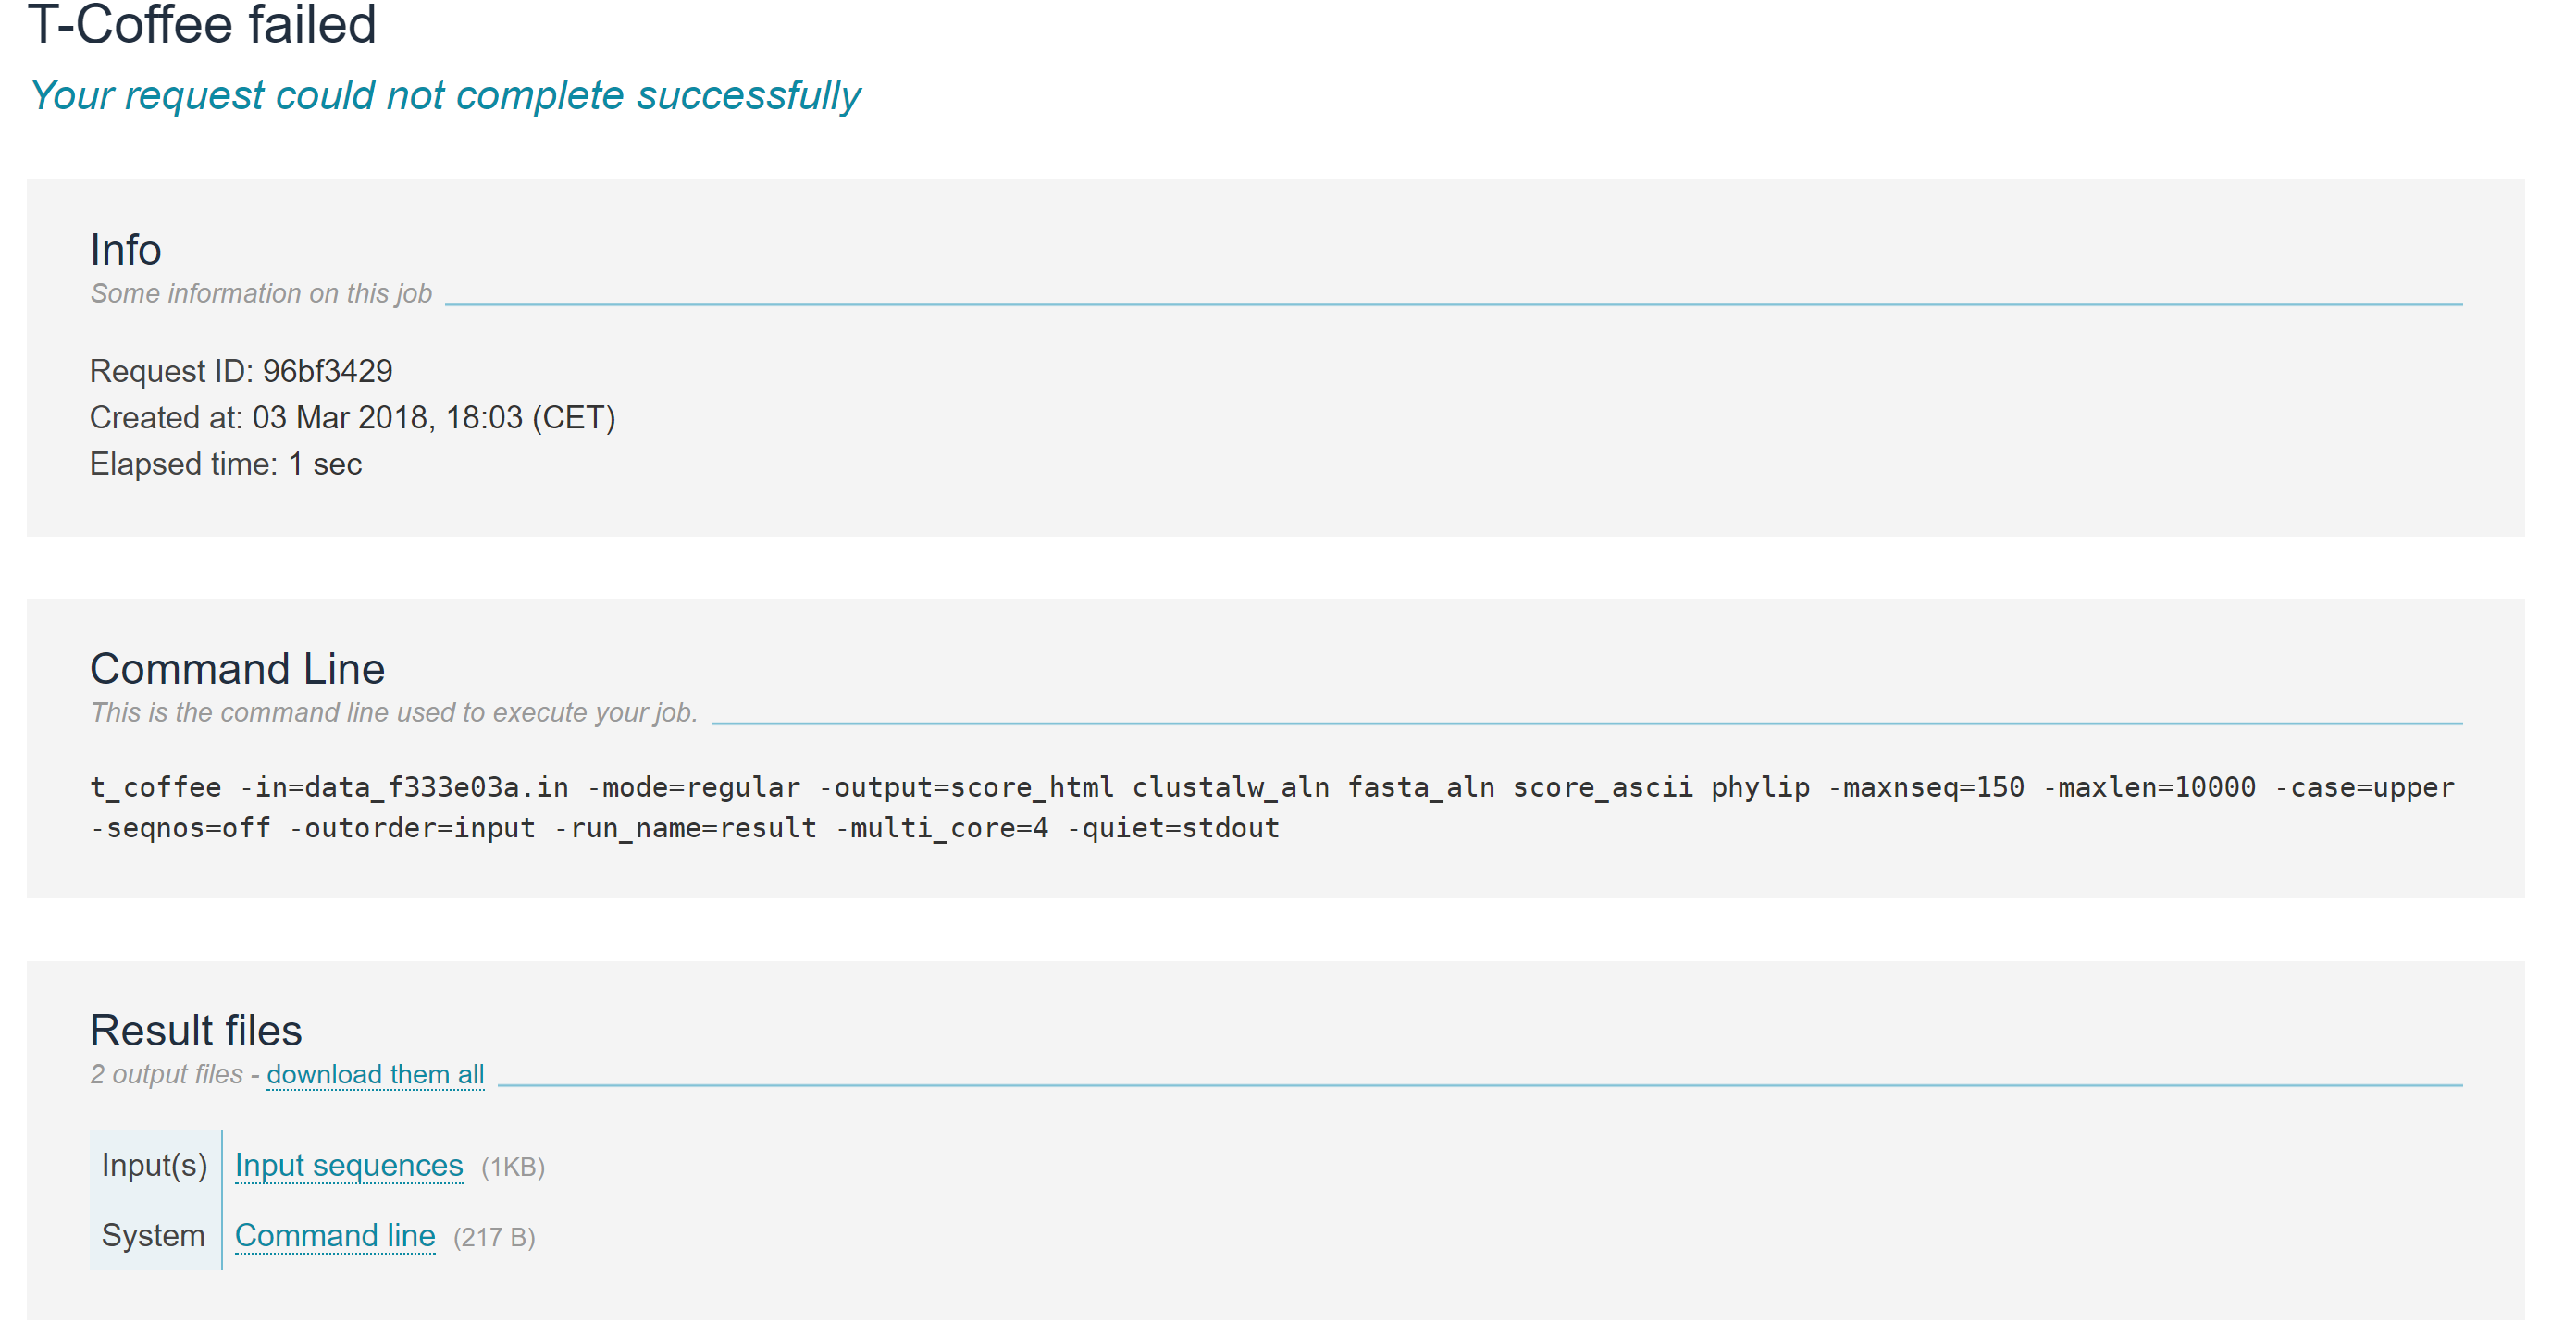
\includegraphics[width=1.2\textwidth]{failed_tcoffee.png}
\caption{Failed T-coffee run}
\label{figure:failedTcoffee}
\end{figure}

\section{UniProt}
Q: What does it mean when a protein unreviewed? \newline
\textit{A: An unreviewed protein is one which has been inferred via computational methods from the genomic sequence but has not been validated experimentally or manually reviewed. See \url{https://www.uniprot.org/help/uniprotkb} for a more detailed explanation.} \newline

\section{BLAST and Sequence alignment}
\subsection{Using BLAST}
Q: What does it mean if there is no complete (identical) match to the protein in Blast data base? \newline
\textit{A: There is no Blast database. Blast is an algorithm which can be used to search a number of different databases, for example the non-redundant protein sequences database, or the Protein Data Bank proteins database. Blast can be queried from the UniProt site if one wishes to search all UniProt sequences (\url{https://www.uniprot.org/blast/}). You do not expect to have an exact match when searching for templates as we have specifically assigned proteins with no resolved structure. If you have no exact match when trying to infer the identity of your protein you are probably searching the wrong database (N.B you may have incomplete coverage as you may have been assigned part of a protein however you should observe 100\% identity).} \newline

Q: I have tried using the BLAST search on UniProt using the sequence I have been given but there is no result that gives a 100\% identity so I cannot figure out which protein has been assigned to me. The search results don't appear to indicate a particular protein. \newline
\textit{A: If there is not a sequence with 100\% identity when identifying the protein even on UniProt, you should still be able to infer the function/identity of the protein from the closest hit. You may mention that there is no exact hit in the discussion.} \newline

Q: How can Blast help in terms of making comparison of two different templates when the two are both hand-picked from blast because they seems to have roughly equally highest quality of alignment to the query sequence. \newline
\textit{A: The E value, coverage and identity should be used to compare templates selected from BLAST. In some cases two templates will have similar such values and thus other factors, such as the resolution of the template can be used. Templates can also be evaluated retrospectively based on the quality of resulting models.} \newline

Q: When I put my query sequence under BLAST, I only get 2 alignments from BLAST. Neither alignment produces a model in SWISS-MODEL when aligning with the query sequence. The first alignment from BLAST contains X's in the FASTA sequence so I thought I would BLAST it in uniprot, and got the same sequence but with M's instead of X. Even with this new sequence I am still unable to produce any type of model. \newline
\textit{A: Some students stumbled across template structures in which non-standard residues (i.e. amino acids other than the 20 standard ones) are found. These residues do occur in certain PDB structures in relation to the particular protein or the methods from which the protein samples are prepared etc. These residues pose difficulty to servers like SWISS-MODEL (and indeed some more advanced modelling packages as well) in which codes other than the standard amino acid codes are not recognised. One way of getting around the problem is to edit the alignment such that the bits of template (and the aligned query) with the non-standard residue is deleted before submitting to the modelling server. \\
We believe this will not be the issue for the vast majority of students, and we so far have not seen any assigned query that could not be modelled if students follow all the instructions and steps we have covered in the tutorials.}  \newline


Q: I have performed a BLAST search and got 100\% match with the part of the protein (using nr database). However, when I used BLAST PDB database, I have got other proteins with 54\% match or less. Do we choose PDB proteins as templates to align them with our query sequence or do we align query sequence with the 100\% match protein (in T-Coffee and BLAST)? \newline
\textit{A: We had a dedicated discussion (especially in the Week 3 tutorial) of which database to BLAST against in different scenarios, and the steps and considerations for template selection has been the focus of the two tutorials on homology modelling. These considerations and steps are explicitly documented in the tutorial slides with comprehensive screenshots. Please consult the tutorial slides to clear your confusion.} \newline 

Q: I was wondering if we have to use the PDB database in our BLAST search (as detailed in the instructions), as I have noticed some questions asking about 100\% identity, which is not obtainable using this database for my FASTA sequence. If I use the non-redundant protein sequences as my database, I receive a hit of 100\% identity, whereas using PDB, the max hit I receive is 35\% identity. \\ Could you please clarify which database we can use, and why, if possible? \newline
\textit{A: The choice of database to BLAST against was explicitly discussed and included in the slides for Tutorial 3. Please also consult similar Q\&A in this document. These should be sufficient to clear confusions (if any) concerning this issue.} \newline


Q: If the BLAST alignment is the best alignment (compared with T-Coffee) how do we use this in alignment-mode homology modelling? \\
As the download from BLAST only downloads the complete/partial sequence of the template, and not the alignment of the template with the query sequence, inputting this file in SWISS-MODEL returns the error "From the sequences you uploaded, no matching templates could be found in the SWISS-MODEL Template Library." \\
Given I can see my alignment in the SWISS-MODEL template library, I know it exists. \\
Is there a way to download the actual alignment from BLAST? \newline
\textit{A: According to the instruction sheet and our tutorials, we did not require students to download BLAST alignments nor to directly input an alignment from BLAST into SWISS-MODEL. Instead BLAST hits are aligned to the query sequence using T-coffee as you clearly have already done. \textbf{BLAST is a search tool but not an alignment tool.} \\
Nevertheless It is possible to download blast alignments (that are, of course, only pairwise alignments). When you scroll the results at the bottom of the search you find a screen like this (Figure \ref{figure:blastDl}), and you have a panel with a lot of option with the format you can save the alignment.} \newline
\begin{figure}[!ht]
\centering 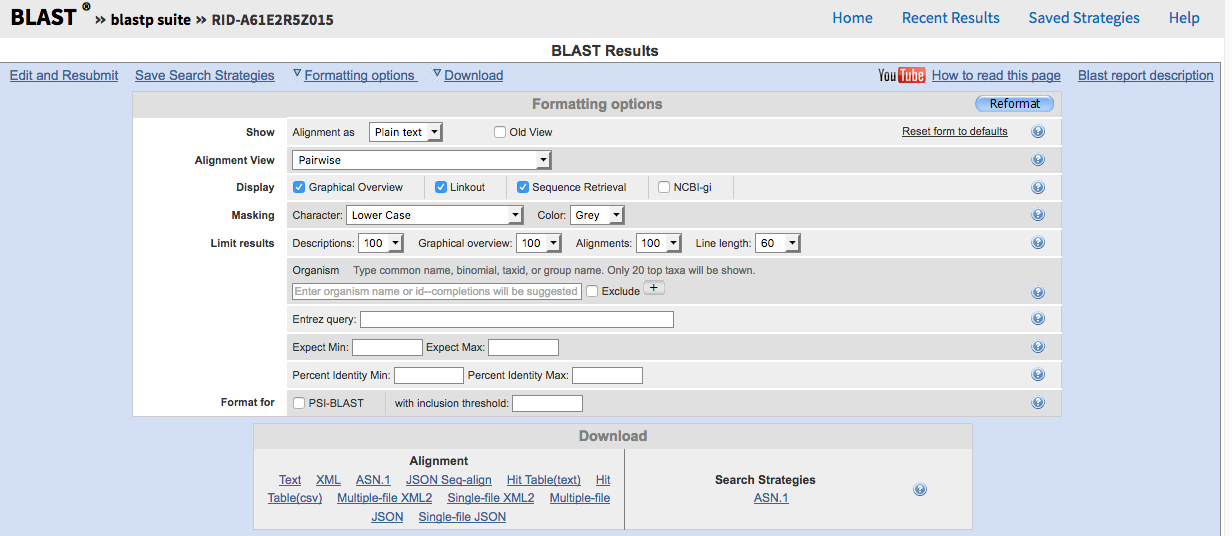
\includegraphics[width=1.2\textwidth]{blast_dl.png}
\caption{Download BLAST alignment}
\label{figure:blastDl}
\end{figure}


\subsection{Comparing alignments}
Q: Which type of metrics can I use to compare BLAST alignments to T-coffee alignments? Both algorithms give scores which are applicable only within the given algorithm, how to compare two different alignments (T-coffee vs BLAST)? \newline
How to compare T-coffee alignments with Swiss Modeller alignments? \newline
\textit{A: Alignments can be compared by looking at the number of exact matches, similar matches and mismatches, as well as gaps. It should be obvious if there are any large differences where, for example gaps are placed in different positions in the alignment. } \newline


Q: Can T-coffee results be used for evaluation straight away? Or does it have to be processed using Swiss model? \newline
\textit{A: The quality of the alignment can be seen from the T-coffee output, however although this plays an important role in determining model quality it is not the only factor. Therefore you should also evaluate your model using the methods described in the tutorial slides (Swiss-model quality scores, Molprobity, alignment of model and template structures in pymol).} \newline


Q: I uploaded my query sequence and chosen template (the one from blast) into tcoffee and I got an alignment score of 100. Should I pick another template from Blast with lower query coverage? \newline
\textit{A: Please exert your own judgement in this case. As we have mentioned in other posts in this forum and in the instruction sheet for this assignment, we  expect students to demonstrate in their essay that they are able to \textbf{compare and discuss} the results they obtained under different modes of SWISS-MODEL and different template structures.} \newline


Q: I would like to know if I should put the t-coffee alignment results in the result analysis section (it helps to choose the template for modeling) or should I put it in the evaluation (treat it as an evaluation of the alignment)?  \newline
\textit{A: What matters is that your results and discussions are clearly conveyed in the essay. Any treatment which you think will contribute to the best readable format for your essay is welcome. } \newline

Q: if the automated mode of SWISS-MODEL and the BLAST search have the same best templates, will handing the BLAST FASTA files to align with t-coffee and then model with SWISS yield different resulting models with the automated mode (because my final models and SWISS reports are the same and I don’t know if it should be the case)? \newline
\textit{A: If the same templates are used and the t-coffee alignment is identical to the Swiss Model alignment, the resulting models should be identical. We suggest you make at least one model using a different template to that chosen by Swiss Model.} \newline

\section{Modelling using SWISS-MODEL}
Q: Are you asking us to do automated homology modelling and manual homology modelling on 1 TEMPLATE sequence and compare the SAME model produced from both? Or do automated homology modelling on 1 Template sequence and manual homology modelling on another template sequence and compare them? \newline
\textit{A: The latter. As we have been doing these all the time in the tutorials, the idea is to compare template selection in the two modes, so if you do have different templates selected in the two modes, please generate your models using the different templates and compare them. \\ Please note that using the same template (and presumably very similar alignments) in the two modes will probably give you nearly-identical models that gives you little to discuss and compare in your essay. \\ Always state clearly, for each model you generated, the "mode" and procedure you have taken, and the template on which the model is based.} \newline

Q:  When choosing models should I not pick the first choice as I heard that it is bad scientific practice? \newline
\textit{A: At no point we have suggested choosing the top hit is a bad scientific practice. Instead, we discussed the reasons and criteria to rank and judge templates. This should also be what you should do in your essay, explaining the scientific reasons and rationale behind your choice of the templates/models.} \newline

Q: what is oligo-state in the SWISS-model, as it mentions that “It is only possible to build a monomer. Not every chain of the biounit will be used to build a model.” \newline
\textit{A: The oligo-state refers to the modelling of protein-protein complexes. For this assignment you are only required to model a monomer. } \newline

Q: if the protein is known for its conformational change in ligand-binding, should I consider also the binding ligand in the template? \newline
\textit{A: Ligand binding and associated conformational changes could certainly form an interesting point for discussion.} \newline

\subsection{Automated modelling}
Q: How many automated models I should make? Which rational criterion I should use here? \newline
\textit{A: a number sufficient for discussion. A minimum of one in automated mode in addition to those created in alignment mode. \textbf{You are not marked only by the number of models you have produced/considered, but more importantly by the quality of your description of what you have done and the discussion of your results.}} \newline

Q: When conducting automated homologies I input my query into the 'Sequence' part of swissmodel and then it gave me quite a few templates to choose from. Should I pick two templates from this stage and compare the two? Or, should I choose one template from this stage and then compare it with the templates they generate when I input my query and my chosen template (from tcoffee alignment) into target-template alignment? \newline 
\textit{A: It is really your decision as to how many to choose. As we have mentioned previously in this forum, there is no hard restrictions as to how many models to pick from the two modes of SWISS-MODEL. The key is you are able to show that you have understood how to use the server for modelling, and that you are able to evaluate and compare your templates and models.} \newline

\subsection{SWISS-MODEL Alignment-mode}
Q: I would like to ask whether I should not use a particular template after I submit it to SWISS model alignment mode and it shows that "Template identifier not recognized and sequence not found in the SMTL”?
\textit{A: Please make sure the template is identified through the BLAST procedure against the correct database. If yes, also make sure that you have followed the steps covered in the tutorial, specifically on checking whether the template identifier (the line that starts with ">" in your FASTA file) conforms to what we suggested in the slides. } \newline

Q: Swiss model does not work for my sequences, it says "target sequences must be unique". Is it because my query is identical to the template? And what should I do if my query sequence is identical to any templates I would select on the BLAST. \newline
\textit{A: This should not have happened. When it comes to template selection through BLAST, this should not be what you expect, as detailed in the Tutorial slides. Please make sure you are searching against the correct database when you are identifying your templates. Remember that the whole point of homology modelling is to find a homologous protein with an experimentally solved structure to model your query sequence (for which you have no structural information) - if you have a 100\% identical template, there is no point at all to do modelling! } \newline



\section{Model evaluation}
Q: How to quantify different MolProbity metrics? How to assign a weight to each category? Is model with, say, two “yellow” scores better than a model with one “green” and one “red”?  What is the MolProbity equivalent of QMEAN (in Swiss Model)? \newline
\textit{A: Please discuss metrics. At no point has it been suggested that MolProbity provides scores which are equivalent to Swiss Model. You are not being asked to assign a weight to each category.} \newline

Q: For automated homology modelling, I have picked two models but cannot find a definitive answer in which is better. Would it be better for analysis to pick two drastically different models with different identities? Or models with similar/same identities, for example the two models I have selected have an identity of 25.37, and have the same QMEAN of 0.58 but different GMQEs at -3.64 and -3.75 respectively. What is GMQE a measure of and is a higher/lower one better in comparison? \newline
\textit{A: you are supposed to study the output of Swiss Model and the meaning of the plots. Please refer to the tutorials: \\
\url{https://www.youtube.com/watch?v=W2Sy3ZUjE88} \\
\url{https://www.youtube.com/watch?v=XDbv1OQ9GWI} \\
\url{https://www.youtube.com/watch?v=lfZRUZn2UQc} \\
\url{https://www.youtube.com/watch?v=WdzHllIay6U} \\
Then you will have to use PERSONAL CRITICAL observation in the discussion of the results.} \newline

Q: The best model from automated homology on SWISS-PLOT (taking into consideration QMEAN GMQE etc), happens to be the same model as my target-template alignment model. Would it be acceptable to discuss that two homology techniques produced the same one? Or should I pick another model from automated homology to compare with my target-template model? \newline
\textit{A: Please exert your own judgement in this case. As we have mentioned in other posts in this forum and in the instruction sheet for this assignment, we  expect students to demonstrate in their essay that they are able to \textbf{compare and discuss} the results they obtained under different modes of SWISS-MODEL and different template structures.} \newline


Q: I have found models in Modbase for my query sequence, but I am unable to compare these models in MolProbity as the coordinates available for download are not accepted as being in PDB format. \\
On further research into the format given in ModBase, I found:
"Coordinate file for the model in the PDB format. The "fifth column" (which normally contains B-factors or order parameters) contains the Modeller error profile. " \\ 
Is this the reason why MolProbity is not accepting my file? I have other ways to compare the models but knowing how to directly input the file to see the MolProbity score would help with my comparison. I could input the coordinates of the template from which the model is based on (which I have done), but this gives me no information about my query sequence (only the template sequence), thus a comparison with models based on my query would not make sense. \newline
\textit{A: Indeed that might be the reason MolProbity is not accepting the Modbase pdb file. There are indeed ways to programmatically clean the pdb file, but this is certainly beyond the scope of what your are expected to do. I will not recommend putting more time into this procedure. \\ 
It is always acceptable if this is clearly described in your essay why you can/cannot do something if this case is specific to your protein/models (like yours).} \newline


\section{Protein domains and evolution}
Q: How can domain structure be determined from Treefam?  \newline
\textit{A: Domain structure cannot be determined using Treefam although domain annotations exist in the Treefam database. Treefam allows one to explore phylogenetic relationships. Pfam or InterPro should be used to infer protein domains. } \newline

Q:  Why the TreeFam button is inactive for my protein and what should I do to perform the TreeFam analysis in such a case? \newline
\textit{A: Search PFAM using the Uniprot ID or Uniprot ID of closest hit, rather than searching with sequence. The TreeFam button should become active. If not, an alternative to access the TreeFam entry of a protein is to go to Uniprot. TreeFam should be one of the phylogenetic databases listed on the UniProt results page. \\ 
If everything doesn't work (consult also the next Q\&A), I suggest that you state that a TreeFam analysis was not possible for your protein, describe clearly the steps you have attempted in your essay, and discuss results regarding the evolution and conservation of domains contained in your sequence (Pfam can be a starting point for this). You can also go back to discuss results regarding domain architecture and homologues of your protein that you find interesting from the other sequence and protein database searches. } \newline

Q: I tried to search the sequence of my protein via \url{http://www.treefam.org/search/sequence}. I am not sure if that is the correct method to perform a TreeFam? If yes, there are more than one TreeFam hits appear. I don't know which one should I choose to use and discuss in my essay. (see screenshots (Figure \ref{figure:treefamSearch}))
\textit{A: Your method of performing a sequence search at TreeFam is indeed acceptable. With regards to which TreeFam hit(s) to discuss, you are certainly not expected to discuss every single possible hit; judging from your screenshots I believe you can make a decision based on the statistics of the hits. There are no limits (both minimum and maximum) as to how many TreeFam results you should discuss, the important thing is again you justify if you filter results in your discussion and comparison, and perhaps reflect on the possible reasons why the web-servers return these results for this particular protein.} \newline
\begin{figure}[!ht]
\centering 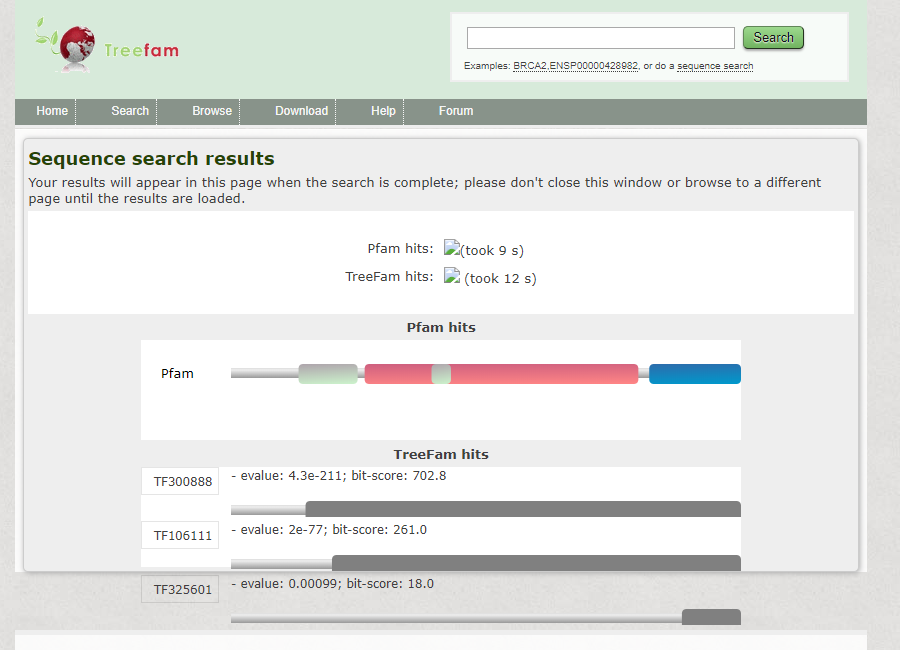
\includegraphics[width=1.2\textwidth]{treefam_search.png}
\caption{Searching TreeFam}
\label{figure:treefamSearch}
\end{figure}

Q: On interpreting TreeFam output: What is the difference between the green circle nodes and the red triangle nodes in the TreeFam? What is expected of the discussion of TreeFam results? \newline
\textit{A: To the best of my knowledge, red symbols should represent duplication events, and green ones for speciation. According to our instructions to the assignments, it would be very sufficient if you are able to discuss generally the TreeFam gene tree, and, more importantly, similarities and differences in \textbf{domain architectures} across members of the gene family - the emphasis here is to discuss any evolutionary information you find interesting about your assigned protein, and integrate these information to reflect on its function and perhaps on the template selection process when you generate your models.} \newline

Q: Any useful online references / tutorials for TreeFam? \newline
\textit{A: there are not many good TreeFam resources online, the best one so far I can find are the papers associated with the TreeFam database and this widget they developed to visualise gene trees, but both of them are rather technical and not strictly on visualisation and the interpretation of results: \\
\url{https://f1000research.com/articles/3-49/v1} (On the visualisation widget) \\
\url{https://academic.oup.com/nar/article/42/D1/D922/1045764} (On the treefam database) \\
I believe these will be (very) extended reading if you are interested in the database and the visualisation, but \textbf{for the sake of the assignment and interpreting the results it is not necessary to refer to these references.}} \newline

%\begin{center}
%\begin{tabular}{ l l }
% \hline
% a & w\\ 
% b & x\\  
% c & y\\   
% d & z\\
% \hline   
%\end{tabular}
%\end{center}
 
\begin{center}
\textsc{END OF DOCUMENT}
\end{center}

\end{document}
